\documentclass{beamer}
\usetheme{CambridgeUS}



\usepackage{enumitem}
\usepackage{tfrupee}
\usepackage{amsmath}
\usepackage{amssymb}
\usepackage{gensymb}
\usepackage{graphicx}
\usepackage{txfonts}

\def\inputGnumericTable{}

\usepackage[latin1]{inputenc}                                 
\usepackage{color}                                            
\usepackage{array}                                            
\usepackage{longtable}                                        
\usepackage{calc}                                             
\usepackage{multirow}                                         
\usepackage{hhline}                                           
\usepackage{ifthen}
\usepackage{caption} 
\captionsetup[table]{skip=3pt}  
\providecommand{\pr}[1]{\ensuremath{\Pr\left(#1\right)}}
\providecommand{\cbrak}[1]{\ensuremath{\left\{#1\right\}}}
\renewcommand{\thefigure}{\arabic{table}}
\renewcommand{\thetable}{\arabic{table}}                                     

\title{AI1110 \\ Assignment 6}
\author{Sai Pradeep \\ AI21BTECH11013}
\date{\today}


\begin{document}
	% The title page
	\begin{frame}
		\titlepage
	\end{frame}
	% The table of contents
	\begin{frame}{Outline}
		\tableofcontents
	\end{frame}
	% The question
	\section{Question}
	\begin{frame}{EXAMPLE 5.28}
Q:-	 We shall show that the characteristic function of an $N(\eta,\sigma)$ random variable x equals $\Phi_x(\omega)=exp(j  \eta  \omega-\dfrac{1}{2}  \sigma^2  \omega^2)$
\end{frame}
	
	% The solution
	\section{Solution}
	\begin{frame}{Solution}
The random variable $x=\dfrac{x-\eta}{\sigma}$ is N(0,1) and its moment function equals 
\begin{align}
\Phi_z (s)&=\int_{-\infty}^{\infty}\dfrac{e^{z \times s} \times e^{\dfrac{-z^2}{2}}}{\sqrt{2 \times \pi }}dz
\end{align}
\begin{align}
s \times z-\dfrac{z^2}{2}&=-\dfrac{(z-s)^2}{2}+\dfrac{s^2}{2}  \\
\Phi_z (s)&=e^{\dfrac{z^2}{2}} \times \dfrac{1}{\sqrt{2\pi}} 
\int_{-\infty}^{\infty}\dfrac{e^{-(z-s)^2}{2}}{\sqrt{2 \times \pi }}dz  \\
\text{Since,} \dfrac{1}{\sqrt{2\pi}} 
\int_{-\infty}^{\infty}\dfrac{e^{x^2}{2}}{\sqrt{2 \times \pi }}dx &=1\\
\label{eq:5}
\Phi_z (s)&=e^{\dfrac{z^2}{2}}
\end{align}
\end{frame}
\begin{frame}{Computation}
As we know that, if y=ax+b then $\Phi_y (w)=e^{jbw} \Phi_x (a \omega)$\\
Since, $x=\sigma \times z + \eta$ \\
\begin{align}
\label{eq:6}
\Phi_x (w)=e^{jw \eta} \Phi_z (\sigma \omega)\\
\Phi_z(j \omega )=\Phi_z(w)
%From equation e ^-w^2
\end{align}
\text{From equation \eqref{eq:5}}    
\begin{align}
\label{eq:8}
\Phi_z (\sigma \omega)=e^(- \dfrac{\sigma^2 \omega^2}{2})
\end{align}
\text{From equations \eqref{eq:6} and \eqref{eq:8}}  
\begin{align}
\Phi_x (w)=e^{jw \eta} \times e^(- \dfrac{\sigma^2 \omega^2}{2})\\
\Phi_x (w)=e^(jw \eta - \dfrac{\sigma^2 \omega^2}{2})
\end{align}
\end{frame}
\begin{frame}{Conclusion}
Hence proved that the characteristic function of an $N(\eta,\sigma)$ random variable x equals $\Phi_x(\omega)=exp(j  \eta  \omega-\dfrac{1}{2}  \sigma^2 \omega^2)$
\end{frame}
\section{Graphs}
\begin{frame}{}
\begin{figure}[htb!]
    \centering
    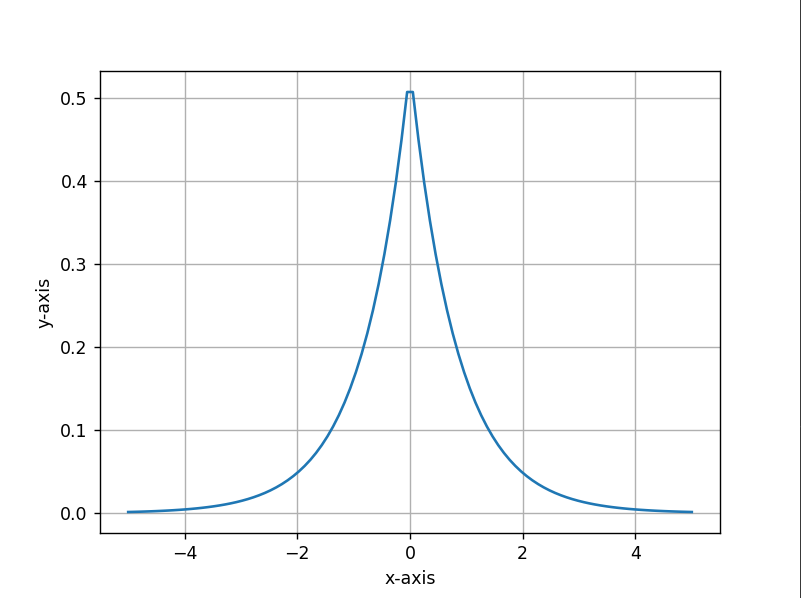
\includegraphics[width=8cm]{figures/fig1.png}
    \caption{}
    \label{fig:my_label}
\end{figure}
\end{frame}

\end{document}
